%%%%%%%%%%%%%%%%%%%%%%%%%%%%%%%%%%%%%%%%%%%%%%
%                insertmeeting
% 1) Title (something creative & funny?)
% 2) Date (MM/DD/YYYY)
% 3) Location (ex. Hagerty High School)
% 4) People/Committees Present 
% 5) Picture 
% 6) Start Time & Stop Time (ex. 12:30AM to 4:30PM)
%%%%%%%%%%%%%%%%%%%%%%%%%%%%%%%%%%%%%%%%%%%%%%
\insertmeeting 
	{FLL Flight Check} 
	{09/09/21}
	{Hagerty High School}
	{Annika, Clayton, Falon, Jensen, Nathan, Rose, Samantha}
	{Images/RobotPics/robot.jpg}
	{2:30 - 3:30}
	
\subsection*{Outreach}
\noindent\hfil\rule{\textwidth}{.4pt}\hfil
\subsubsection*{Goals}
\begin{itemize}
    \item Prepare for upcoming fll meetings 

\end{itemize} 

\noindent\hfil\rule{\textwidth}{.4pt}\hfil

\subsubsection*{Accomplishments}
During this meeting, we started planning for our upcoming FLL meetings. These meetings will occur almost every week through April, and, as a part of the hagerty robotics junior program, will be led entirely by 4717 members. We have 3 different levels of FLL that we mentor including Discover, Explore, and Challenge with a total of more than 30 kids! We divided them up into 1 Discover group, 3 Explore teams, and 2 challenge teams, all of which will meet after school on Fridays, with challenge members also meeting on tuesdays.
As our first meeting will take place tomorrow, we needed to get more organized and come up with a more solid plan for each of the levels of FLL. To do this, we broke up into groups depending on if we were mentoring discover, explore or challenge kids. We already had some ideas of what we wanted to do at the first meeting and we already gathered session slides created by FIRST for all 3 levels of FLL. We decided to use the introduction slideshows for the explore and challenge levels, but we changed them up to be more clear and engaging for our members (image 1). Once we made plans for tomorrow’s, we made a material list of what we would need, including all of the lego boxes for the discover and explore levels, and ipads, the challenge mats, and challenge game pieces for challenge. We also created an agenda for fll challenge that could be sent to parents detailing what we would be doing at this meeting (image 2). 
Once we had done all of this, we felt prepared for tonight, and continued to make plans for next week. For FLL challenge, we are planning to start off the season by teaching the members, most of whom have little experience with FLL, the basics of building and programming with the ev3. As we have in years past, we will start with a riley rover, a simple lego base robot, and ensure that all of the members are brought up to speed on how to program and build. Building the riley rover and learning to program it through a course will be the main focus of next week’s challenge meetings, but we also will find time to give a presentation about core values and gracious professionalism, which are important not just in FIRST, but in members’ everyday lives. As for Explore and Discover, we plan on introducing the kids to the different methods of transportation in accordance with this year’s theme. We plan on allowing them to use legos to build their own design of a form of transportation.
 

\begin{figure}[ht]
\centering
\begin{minipage}[b]{.50\textwidth}
  \centering
  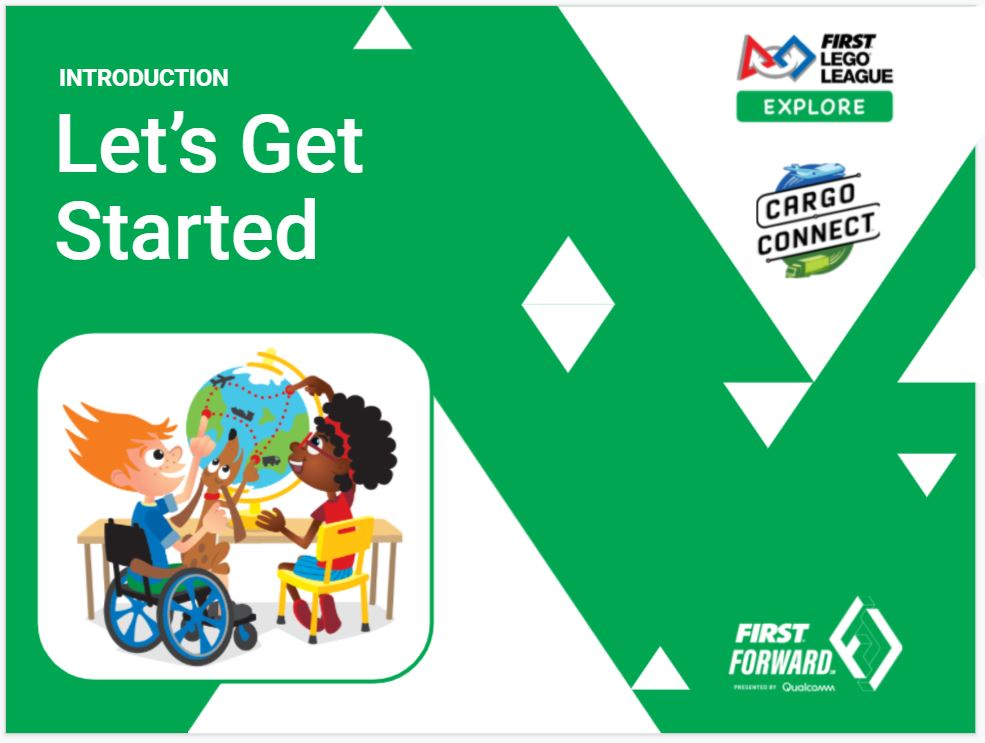
\includegraphics[width=0.8\textwidth]{Meetings/September/09-09-21/9-9-21_Outreach_Image1 - Nathan Forrer.JPG}
  \caption{Our redesigned slideshows we used to teach younger students.}
  \label{fig:pic1}
\end{minipage}%
\hfill%
\begin{minipage}[b]{.50\textwidth}
  \centering
  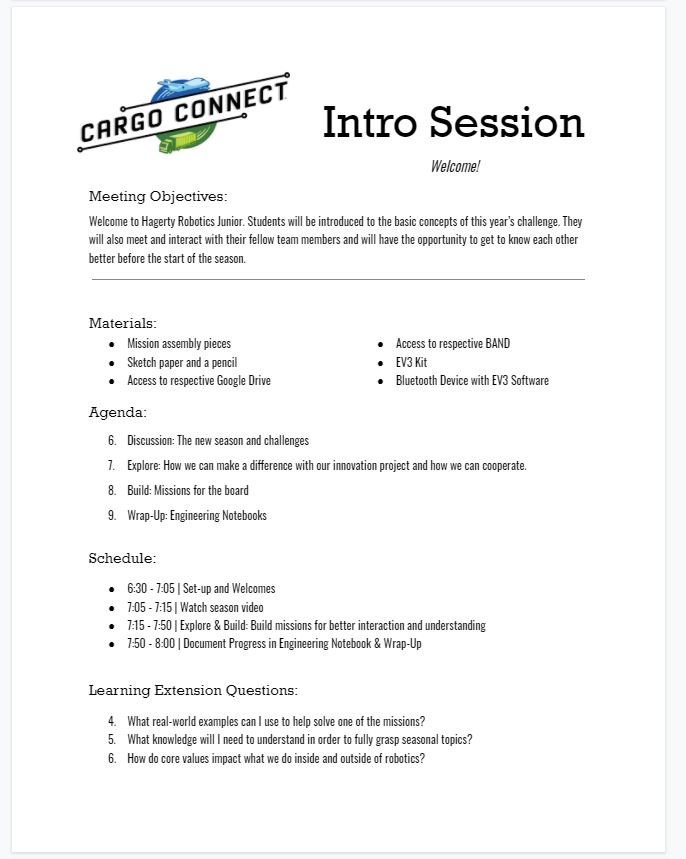
\includegraphics[width=0.8\textwidth]{Meetings/September/09-09-21/9-9-21_Outreach_Image2 - Nathan Forrer.JPG}
  \caption{A screenshot of the information we covered at today's meeting.}
  \label{fig:pic2}
\end{minipage}
\end{figure}

\subsection*{Software}
\noindent\hfil\rule{\textwidth}{.4pt}\hfil
\subsubsection*{Goals}
\begin{itemize}
    \item Figure out why the Robot is not strafing properly

\end{itemize} 

\noindent\hfil\rule{\textwidth}{.4pt}\hfil

\subsubsection*{Accomplishments}
During this meeting, we wanted to figure out why the robot was not strafing properly. Our mentor, Mr. Don Harper, suggested Logging the encoder values in Logcat in Android studio. We would do so by using the Log.i() implementation already in Java. This would allow us to be able to find out if the motors themselves were going at different speeds. We later found out that they were going at different speeds by just a tad. We then switched the power no matter where the joystick is to automatically 1 or -1 by using Math.floor() if a negative value was recorded on the Joystick and Math.ceil() if a positive value was recorded. The reason as to why we thought this would help is because the encoder values might have been off since different values on each side of the joystick could have been recorded. This, however was not the problem as the encoder values were still off. Even though the Mecanum drive was still going in an arc, we were glad to have finally found the root of the problem and are hopeful to fix it soon.





